\documentclass[conference]{IEEEtran}
\usepackage{graphicx}
\usepackage{epstopdf}
\usepackage{array}
\usepackage{multirow}
\usepackage{multicol}
\usepackage{empheq}
\usepackage{algorithm}
\usepackage{algorithmicx}
\usepackage{algpseudocode}
\usepackage{amsmath}
\renewcommand{\algorithmicrequire}{ \textbf{Input:}} %Use Input in the format of Algorithm
\renewcommand{\algorithmicensure}{ \textbf{Output:}} %UseOutput in the format of Algorithm
% correct bad hyphenation here
\hyphenation{op-tical net-works semi-conduc-tor}
\begin{document}
\title{Parsing Tables from EDGAR with Python \\and Its Dockerization}
%
% author names and affiliations
\author{\IEEEauthorblockN{Jiali Cheng$^{1}$}
\IEEEauthorblockA{$^{1}$Graduate School of Engineering, Northeastern University, Boston, USA}
}
% make the title area
\maketitle
\begin{abstract}
We use Python to access data from EDGAR, the Electronic Data Gathering, Analysis, and Retrieval system. Given a company ID, called CIK, and an Access Number, called acc-no, an URL to this HTML file is generated. We locate to the 10Q file and extract all the tables and save them as CSV(Comma Separated Values) files. Then we dockerize this pipeline so that it can be used for any websites, not only restricted to IBM.
\end{abstract}
\begin{keywords}
Parse Tabels, HTML, EDGAR, Python, Docker
\end{keywords}
\IEEEpeerreviewmaketitle
%
%Introduction
\section{Introduction}\label{i}
\indent The Electronic Data Gathering Analysis and Retrieval (EDGAR) system is run by Office of Information Technology, U.S. Securities and Exchange Commission. performs automated collection, validation, indexing, acceptance, and forwarding of submissions by companies and others who are required by law to file forms with the SEC. The database is freely available to the public via the Internet (Web or FTP).
\\
\indent In this paper we focus on parsing the tables in the 10Q file of each company. And we introduces a way that given a CIK (company ID), automatically generates the URL (Uniformly Resource Location) to the 10Q file and parse all the tables to save to a CSV file. We then build this pipeline into a Docker image so that it can run on other PCs or laptops. 
\\
\indent Parsing tables have always been a hot topic and a useful tool for data collection. We use 
\\
\indent The remainder of the paper is organized as follows. In Sect.~\ref{ii} we briefly go through the objectives and expectations of the TableParser package and provide an overview of it. Then we detail the design of this package in Sect.~\ref{iii}. Sect.~\ref{iv} presents the results and analysis of the algorithm and code. And in Sect.~\ref{vii} we conclude the report.
\\
%TableParser
\section{Exploratory Data Analysis}\label{ii}
\indent According to the issues addressed in Sect.~\ref{ii}, we develop a package called TableParser. It basically follows the processing order shown in Fig. ~\ref{flowchart}. Given an Accession Number, we can easily generate the URL of its files on the EDGAR system. And we use regular expression to locate to the 10Q file of this company, which is the target of our parsing job. Then we call the read\_html function to parse the tables out. We clean the noisy data and write it to a CSV file.
\\
%
\begin{figure}
\centering
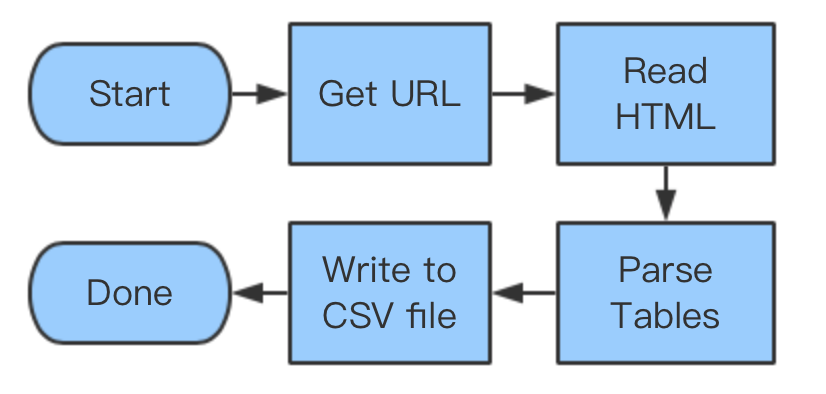
\includegraphics[width=3.8in]{flow1.png}
\caption{The processing flowchart}\label{flowchart}
\end{figure}
%
%Algorithm
\section{Data Preprocessing/Wrangling}\label{iii}
depends.
i) missing value???????????????????????
ii) missing value????????????????????????????????????????????????????????????????????????
iii) missing value as another occasion, and assign them a value.
\section{Feature Engineering}\label
Feature selection is a process where you automatically select those features in your data that contribute most to the prediction variable or output in which you are interested.
Having too many irrelevant features in your data can decrease the accuracy of the models. Three benefits of performing feature selection before modeling your data are:
Reduces Overfitting: Less redundant data means less opportunity to make decisions based on noise.
Improves Accuracy: Less misleading data means modeling accuracy improves.
Reduces Training Time: Less data means that algorithms train faster.
Many kernels posted for this competition doesn't use one hot encoding for many variables which I believe should be treated as such. For example, regionzipid (i.e. zip code) is not exactly a numerical variable and there isn't ordinal relationship between two zip codes. Same goes for other variables such as airconditioningtypeid, architecturalstyletypeid etc.

When I try one hot encoding on those variables and use XGB, my scores are worse than not using one hot encoding. 
\\
%
\section{Model Selection and Training}\label{v}
\indent Linear Regression

R-squared, also called coefficient of determination, indicates the fitting degree of the model to the real data. In one linear regression, r-squared equals the square of Pearson product moment correlation coefficient.

\indent Random Forest
The sklearn.ensemble module includes two averaging algorithms based on randomized decision trees: the RandomForest algorithm and the Extra-Trees method. Both algorithms are perturb-and-combine techniques [B1998] specifically designed for trees. This means a diverse set of classifiers is created by introducing randomness in the classifier construction. The prediction of the ensemble is given as the averaged prediction of the individual classifiers.
Random Forest has less bias, need to reduce variance. sub models are not weak models.
scale cannot be big since it takes a lot of memory. rf is a black box we don't know what's inside.

\indent Neural Network
%
\section{Model Ensemble}\label{vi}
%
\section{Conclusion}\label{vii}
%
\begin{thebibliography}{1}
\bibitem{NASA's Space}
Liebrecht, P., Schier, J., Bhasin, K., Bibyk, I., Butler, M., Hudiburg, J., Tai, W., Shames, P., NASA's Space Communications Integrated Architecture, Proceedings of SpaceOps 2010 Conference, AIAA, 25-30 April 2010, Huntsville,
Alabama.
\end{thebibliography}
\end{document} 